\documentclass{beamer}

\ifx\narrator\undefined
  \newcommand\narrator{Albert Einstein}
\fi

\ifx\voice\undefined
  \newcommand\voice{Daniel (mac text2speech)}
\fi

\usepackage[author={narration}]{pdfcomment}
\definestyle{note}{icon=Insert,color=red} 
\newcommand{\pdfnarration}[1]{%
\onslide*<\value{beamerpauses}>{\pdfmargincomment[style=note,author=narration]{#1}}%
}

\usepackage{hyperref}
\newcommand{\tinyurl}[1]{\tiny \url{#1} \normalsize}

\newcommand\showpauses{The value of beamerpauses at this point in slide \insertpagenumber\ is: \thebeamerpauses}

\usepackage{amsmath}
\usepackage{tikz, tikz-3dplot, pgfplots} %diagrams
	\usetikzlibrary{calc, hobby, patterns, intersections, angles, quotes, spy, shapes, plotmarks, math, quotes, angles, positioning}

\usepackage{multicol}    %  two columns for problem sections
%\usepackage{picins}      %  to insert small drawings in paragraphs

\renewcommand{\pdfnarration}[1]{}

%Information to be included in the title page:
\title{PORPIDpipeline}
% \subtitle{narrated by  \\  \voice }

\subtitle{\bigskip \url{https://github.com/MurrellGroup/PORPIDpipeline} }

\institute{sponsored by \\ 
Division of Medical Virology, \\
Department of Pathology, \\
University of Cape Town.}

\date{2022}
%\titlegraphic{\includegraphics[width=2cm]{images/Leonhard_Euler.jpeg}}

%\newcommand\pdfnarration[1]{%
%    \pdfmargincomment[style=note,author=narration]{#1} }%

%\pdfnarration{
% [[slnc 2000]]
% In this video we present a modern solution to the Basel problem. 
% [[slnc 2000]]
%}

%\AtBeginSection[]
%{
%    \begin{frame}
%        \frametitle{outline \ldots}
%        \tableofcontents[currentsection]
%    \end{frame}
%}

%\AtBeginSubsection[]
%{
%    \begin{frame}
%       \frametitle{outline \ldots}
%        \tableofcontents[currentsubsection]
%    \end{frame}
%}



\begin{document}

\frame{\titlepage}

\begin{frame}{Outline}
\tableofcontents
\end{frame}

\section{Introduction}


\begin{frame}
\frametitle{ Introduction - UMI sequencing }

\alert<1> 

\begin{multicols}{2}
\includegraphics[width=4cm]{images/overview.png}

 {\em Unique Molecular Identifiers} (UMIs) are short sequences 
 incorporated into each fragment before PCR amplification 
 so as to identify the molecule of origin for each read and to 
 identify PCR duplicates. \bigskip
 
A short (6bp) user selected UMI is affixed during 
cDNA synthesis and identifies the {\em donor}.  \bigskip

A longer (8bp) randomly generated UMI identifies duplicate reads 
originating from the same molecule, these are called {\it amplicons}.

\end{multicols}

\pdfnarration{
[[slnc 1000]]
Unique molecular identifiers, are random barcodes, that are increasingly used to 
confidently identify [[emph +]] samples and duplicates [[emph -]] in 
next generation sequencing experiments,
[[sinc 1000]]
Unique molecular identifiers, can be applied to a wide range of sequencing methods,
 in which an accurate detection of rare mutations is required.
[[slnc 1000]]
}

\end{frame}


\section{Wetlab}

\begin{frame}[fragile]
\frametitle{ Wetlab - reverse transcription }

\alert<1> 


\bigskip
An RNA sample is obtained from a donor. The RNA is
converted to cDNA through one round of reverse transcription using 
a cDNA primer composed of four parts. for example:

\tiny
\begin{verbatim}
    cDNA_primer: CCGCTCCGTCCGACGACTCACTATAacagtgNNNNNNNNGTCATTGGTCTTAAAGGTACCTG
\end{verbatim}
\normalsize

\begin{itemize}
\item[1)] first we have a 25nb receptor that will be used as a binding site in the PCR steps to follow
\item[2)] next we have a 6nb user selected donor barcode shown in lower case
\item[3)] next we have an 8nb random barcode which identifies the cDNA strand to be amplified
\item[4)] lastly we have a 23nb primer that will bind to the RNA upstream of a region of interest, henseforth referred to as the {\em amplicon} (that to be amplified).
\end{itemize}

\pdfnarration{
[[slnc 1000]]
In order to comprehend the pipeline, we must first get an understanding
of the wetlab procedures that are used to generate the sequences for PacBio processing.
[[sinc 2000]]
An RNA sample is obtained from a donor. 
[[sinc 2000]]
The RNA is converted to CDNA through one round of 
reverse-transcription using a primer, such as the one shown in the slide.
[[sinc 2000]]
In this example the first 25 base pairs provide a binding site for subsequent PCR amplification.
[[sinc 2000]]
The next 6 base pairs ( in lower case ) provide a barcode identifying the donor.
[[sinc 2000]]
The next 8 base pairs ( the Ns ) represent a randomly generated barcode that identifies the ampli-con.
[[sinc 2000]]
The last 23 base pairs, on reversal, provide a primer that will bind to the RNA upstream of the ampli-con.
[[sinc 1000]]
}




\end{frame}

\begin{frame}[fragile]
\frametitle{ Wetlab -  cDNA  }

\alert<1> 

The cDNA primer is designed so that, on reversal, the portion after the N's will bind to the RNA strand
upstream from the amplicon.  

\bigskip
The remaining components of the reversed primer {\it hang} off the primer
upstream of the binding site.

\begin{center}
\includegraphics[width=8cm]{images/cDNA_primer-binding.png}
\end{center}

After binding the {\it reverse transcriptase} enzyme 
extends the reversed primer, thus complimenting the RNA to obtain cDNA. 

% \bigskip
% read this \href{https://wikipedia.org/wiki/Complementary_DNA}{\color{green} Wikipedia} article  for more details.

\bigskip
for more details, watch this \href{https://www.youtube.com/watch?v=0MJIbrS4fbQ}{\color{red} YouTube} video.

\pdfnarration{
[[slnc 1000]]
The CDNA primer, is designed so that, on reversal, the portion after the N's will bind to the RNA strand
upstream from the ampli-con.
[[slnc 1000]]
The remaining components hang off the primer, as shown in the diagram.
[[sinc 1000]]
After binding the [[emph +]] reverse-transcriptase-enzyme  [[emph -]] 
extends the primer, thus complimenting the RNA to obtain the CDNA. 
[[sinc 1000]]
}

\end{frame}

\begin{frame}[fragile]
\frametitle{ Wetlab -  PCR first round}

After purification our cDNA  fragments are moved to another instrument for PCR amplification.
All fragment have identical donor barcodes but a unique randomly generated CDNA barcode. 

\bigskip
Two primers are used for the PCR reactions, a new primer called the {\tt sec\_str\_primer}
and the first part of the previous {\tt cDNA\_primer}

\tiny
\begin{verbatim}
    sec_str_primer: TAGGCATCTCCT
    cDNA_primer: CCGCTCCGTCCGACGACTCACTATA
\end{verbatim}
\normalsize

In the first round of PCR, the {\tt cDNA\_primer} does no work  
but the {\tt sec\_string\_primer} binds 
{\bf downstream} of the amplicon in the cDNA. 

\pdfnarration{
[[slnc 1000]]
After purification our CDNA  fragments are moved to another instrument for PCR amplification.
[[sinc 1000]]
All fragment have identical donor barcodes but a unique randomly generated CDNA barcode. 
[[sinc 1000]]
Two primers are used for the PCR reactions.
The one being a new primer, called [[emph +]]  the secondary string primer [[emph -]],
and the other being the first part of the previous CDNA primer.
[[sinc 1000]]
In the first round of PCR, the secondary string primer binds 
downstream of the ampli-con in the CDNA
 complementing the CDNA strand 
to the end of the CDNA primer.
[[sinc 2000]]
}

\end{frame}

\begin{frame}[fragile]
\frametitle{ Wetlab -  PCR continued\ldots   }

\alert<1> 

In the first round of PCR, the DNA polymerase extends the 
{\tt sec\_string\_primer} complementing the cDNA strand 
to the end of the {\tt cDNA\_primer}.

\bigskip
From the second round onwards the {\tt cDNA\_primer} binds upstream
of the donor's barcode and both primers are extended.

\bigskip
If we start the PCA reaction with $N$ distinct cDNA fragments,
each with a unique random barcode, then,  assuming 
successful primer extensions,
round by round amplification will proceed as follows

$$ N \xrightarrow{round(1)} N   \xrightarrow{round(2)} 2N  \xrightarrow{round(3)}  4N  
 \cdots \xrightarrow{round(r)} 2^{r-1} N $$

for an explanation of the PCR process
 watch this \href{https://www.youtube.com/watch?v=c07_5BfIDTw}{\color{red} YouTube} video.


\end{frame}

\begin{frame}[fragile]
\frametitle{ Wetlab -  PacBio   }

\alert<1> 

At the end of the PCR process we have many copies of DNA strands from
the same donor with each strand incorporating both a user specified donor barcode
and a random cDNA barcode from which the strand was amplified.

\bigskip
Samples from different donors and different amplicons are collected for
one PacBio sequencing run.

\bigskip
The PacBio system attaches a circular ligate adaptor at each end of the DNA fragment 
and then sequencing begins by means of a primer that binds to the ligate
and extends many times around the fragment issuing sequencing signals
for each extension base. 

\bigskip
After the sequencing has completed PacBio software performs sequence assembly
and returns the sequences in {\tt fastq} format which gives both the 
sequence bases and a confidence measure for each base sequenced (see next slide).

\end{frame}

\begin{frame}[fragile]
\frametitle{ Wetlab -  PacBio \ldots   }

\alert<1> 

\begin{center}
\includegraphics[width=6cm]{images/PacBioPic.png}
\end{center}

\bigskip
for further elucidation watch this \href{https://www.youtube.com/watch?v=-nOr5B_bF3A}{\color{red} YouTube}
video.

\end{frame}

\section{Snakemake}

\begin{frame}
\frametitle{Snakemake - introduction }

\alert<1> 

{\em Snakemake} is a workflow management system for pipelines that handles:

\begin{itemize}
\item suspension and resumption
\item logging
\item data origins
\item parallelization
\end{itemize}

\bigskip
To use Snakemake, you must decompose workflow into rules.

\begin{itemize}
\item rules define how to obtain output files from input files.
\end{itemize}

\bigskip
{\em Snakemake} will infer dependencies and execution order
from a set of rules stored in a {\tt snakefile}.


\end{frame}

\begin{frame}[fragile]
\frametitle{Snakemake - rules }

\alert<1> 

\begin{itemize}
\item rules are {\em named}
\item rules are {\em indented}
\item there can be {\em multiple named} input and output files.
\item names can incorporate {\em wildcard} parts
\item a rule has a {\em shell script} telling how to generate output from input.
\end{itemize}

\bigskip
\begin{tiny}
\begin{verbatim}
rule sort_and_annotate:
    input:
        a="path/to/{dataset}.txt",
        b="path/to/annotation.txt"
    output:
        "{dataset}.sorted.txt"
    shell:
        "paste <(sort {input.a}) {input.b} > {output}"
\end{verbatim}
\end{tiny}


\end{frame}

\begin{frame}[fragile]
\frametitle{Snakemake - jobs }

\alert<1> 

Dependencies are determined top-down.

\bigskip
\begin{itemize}
\item For a given target, a rule that can be applied to create it is called a {\em job}.
\item For the input files of the job, rules are determined recursively.
\end{itemize}

\bigskip
A job is executed if and only if

\begin{itemize}
\item output file is target and does not exist
\item output file needed by another executed job and does not exist
\item input file newer than output file
\item input file will be updated by other job
\item execution is enforced by command line parameters
\end{itemize}

determined via breadth-first-search of the Directed acyclic graph (DAG) of the workflow.

\end{frame}

\begin{frame}[fragile]
\frametitle{Snakemake - command line }

\alert<1> 

assuming that the workflow is defined in {\tt snakefile}.

\begin{tiny}
\begin{verbatim}
# execute the workflow with target D1.sorted.txt
snakemake D1.sorted.txt

# execute the workflow without target: first rule defines target
snakemake

# dry-run
snakemake -n

# dry-run, print shell commands
snakemake -n -p

# dry-run, print execution reason for each job
snakemake -n -r

# visualize the DAG of jobs using the Graphviz dot command
snakemake --dag | dot -Tsvg > dag.svg
\end{verbatim}
\end{tiny}

\end{frame}

\begin{frame}[fragile]
\frametitle{Snakemake - example }

\alert<1> 

contents of {\tt snakefile}

\begin{tiny}
\begin{verbatim}
DATASETS = ["D1", "D2", "D3"]

rule all:
    input:
        expand("{dataset}.sorted.txt", dataset=DATASETS)


rule sort:
    input:
        "path/to/{dataset}.txt"
    output:
        "{dataset}.sorted.txt"
    shell:
        "sort {input} > {output}"
\end{verbatim}
\end{tiny}

workflow DAG

\bigskip
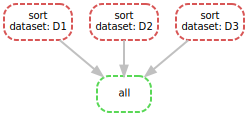
\includegraphics[width=4cm]{images/small_dag.png} 


\end{frame}

\begin{frame}[fragile]
\frametitle{Snakemake - configfile }

\alert<1> 

\begin{small}
Often you want your workflow to be customisable, so that it can easily be adapted to new data. 
For this purpose, Snakemake provides a config file mechanism. 
Config files are specified with the configfile directive.
Snakemake will load the config file and store its contents into a 
globally available {\em dictionary} named {\tt config}.
\end{small}

\bigskip
{\tt config.yaml}
\begin{tiny}
\begin{verbatim}
datasets: 
  D1:
  D2:
  D3:
\end{verbatim}
\end{tiny}

{\tt snakefile}
\begin{tiny}
\begin{verbatim}
configfile: "config.yaml"

rule all:
    input:
        expand("{dataset}.sorted.txt", dataset=config["datasets"])

rule sort:
    input:
        "path/to/{dataset}.txt"
    output:
        "{dataset}.sorted.txt"
    shell:
        "sort {input} > {output}"
\end{verbatim}
\end{tiny}

\end{frame}

\begin{frame}[fragile]
\frametitle{to continue \ldots }

\alert<1> 

For the remainder of this presentation we will describe each
script in PORPIDpipeline and show how to invoke
the script via SnakeMake.

\bigskip
At the beginning of the {\tt snakefile} we have the following instructions 
to parse the {\tt demo} PORPIDpipeline config file shown on the next slide.

\begin{tiny}
\begin{verbatim}
configfile: "config.yaml"
DATASETS = [d for d in config for s in config[d]]
SAMPLES = [s for d in config for s in config[d]] 
\end{verbatim}
\end{tiny}

\bigskip
In the demo config file we have one dataset, {\tt demo}, in which there
are 6 samples (3 donors each with 2 amplicons).

\bigskip
For each sample we specify the primers used and a panel file.

\end{frame}

\begin{frame}[fragile]
\frametitle{to continue \ldots  \ldots}

\alert<1> 

demo PORPIDpipeline  {\tt config.yaml}:

\begin{tiny}
\begin{verbatim}
demo:
  donor_1_REN:
    cDNA_primer: CCGCTCCGTCCGACGACTCACTATAacagtgNNNNNNNNGTCATTGGTCTTAAAGGTACCTG
    sec_str_primer: TAGGCATCTCCT
    panel: "panels/HIV1_COM_2017_5970-8994_DNA_stripped.fasta"
  donor_2_REN:
    cDNA_primer: CCGCTCCGTCCGACGACTCACTATAcactcaNNNNNNNNGTCATTGGTCTTAAAGGTACCTG
    sec_str_primer: TAGGCATCTCCT
    panel: "panels/HIV1_COM_2017_5970-8994_DNA_stripped.fasta"
  donor_3_REN:
    cDNA_primer: CCGCTCCGTCCGACGACTCACTATAggtagcNNNNNNNNGTCATTGGTCTTAAAGGTACCTG
    sec_str_primer: TAGGCATCTCCT
    panel: "panels/HIV1_COM_2017_5970-8994_DNA_stripped.fasta"
  donor_1_GP:
    cDNA_primer: CCGCTCCGTCCGACGACTCACTATAacagtgNNNNNNNNGTATGTCATTGACAGTCCAGC
    sec_str_primer: TTGACTAGCGGAGGCTAGAAGGAGA
    panel: "panels/HIV1_COM_2017_787-3300_DNA_stripped.fasta"
  donor_2_GP:
    cDNA_primer: CCGCTCCGTCCGACGACTCACTATAcactcaNNNNNNNNGTATGTCATTGACAGTCCAGC
    sec_str_primer: TTGACTAGCGGAGGCTAGAAGGAGA
    panel: "panels/HIV1_COM_2017_787-3300_DNA_stripped.fasta"
  donor_3_GP:
    cDNA_primer: CCGCTCCGTCCGACGACTCACTATAggtagcNNNNNNNNGTATGTCATTGACAGTCCAGC
    sec_str_primer: TTGACTAGCGGAGGCTAGAAGGAGA
    panel: "panels/HIV1_COM_2017_787-3300_DNA_stripped.fasta"
\end{verbatim}
\end{tiny}

\end{frame}

\begin{frame}
\frametitle{to continue \ldots \ldots \ldots  }


\alert<1> 

%\begin{multicols}{2}

%The {\tt snakefile} for the PORPIDpipeline pipeline is too long to show in one slide.
The image below is a directed acyclic graph (DAG) of the pipeline
showing all the scripts and the order of execution

\begin{center}
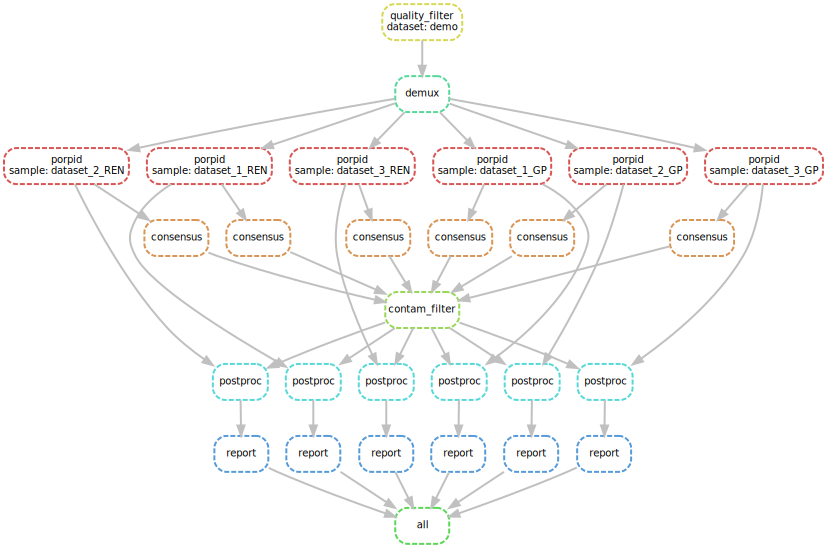
\includegraphics[height=5cm]{images/dag.png}
\end{center}

In the following slides we discuss each script in the pipeline.

%\end{multicols}


\pdfnarration{
 [[slnc 1000]]
 Porpid Postproc is a pipeline of Julia scripts designed to assist with molecular sequence
 extraction from pooled samples. 
 [[sinc 1000]]
 In this example we see six samples each tagged with
 a unique molecular identifier but all pooled for one PacBio sequencing run.
 [[sinc 1000]]
 The pipeline performs demultiplexing of the three samples followed Porpid
 processing of each sample to be run in parallel. 
 [[sinc 1000]]
 In the slides that follow, we will describe each step in the pipeline in more detail.
[[slnc 1000]]
}

\end{frame}

\section{Pipeline}

\subsection{demux}

\begin{frame}[fragile]
\frametitle{ demux }

\alert<1> 

Because PacBio runs are expensive, samples are tagged and pooled for one sequencing run.
This is called {\em multiplexing} and after the sequencing, the sequences generated must be {\em de-multiplexed}.

\bigskip
This {\em de-multiplexing} allows us to separate the full dataset into sample datasets which are more manageable
in size and which can be further processed in parallel.

\bigskip
In the demux script we read the pac-bio dataset in {\em chunks} directly from a zipped file
and then we perform quality filtering and de-multiplexing on each chunk and then we append
each de-multiplexed sequence to the appropriate demux file for that sample.

\end{frame}


\begin{frame}
\frametitle{ demux - quality filtering  }

\alert<1> 

Raw reads from a PacBio sequencing run comprise of DNA fragments with confidence scores
for each nucleotide in the sequence. For example:

\includegraphics[width=10cm]{images/fastq_example.png}

The confidence scores, also known as {\em Phred} quality scores, are integers from 0 to 93, 
encoded using ASCII  characters 33 to 126, and a log scale on the probability of an incorrect call.

\bigskip
To compute the probability $P$ of an incorrect base call we evaluate

\begin{align*}
	P_{incorrect} = 10 ^{- \frac{Q-33}{10} }
\end{align*}

for each ASCII character $Q$ in the quality string. 
\pdfnarration{ 
[[sinc 1000]]
Our starting point is a set of pooled raw reads in fast q format.
[[sinc 1000]]
The confidence scores, also known as {\em Phred} quality scores, 
are integers from 0 to 93,  encoded using ASCII  characters 33 to 126.
[[sinc 1000]]
A log scale is used to encode the probability of an incorrect call.
[[sinc 1000]]
This probability of an incorrect base call, can be computed
using the formula shown.
[[sinc 1000]]
}

\end{frame}


\begin{frame}
\frametitle{ demux - quality filtering \ldots  }

\alert<1> 

In our quality filter we reject fragments who's
mean probability of an incorrect call (error rate) is greater than a user supplied parameter. 

\bigskip
We also reject fragments who's length is either too small or too large 
as specified by user supplied parameters.

\bigskip
In our PorpidPostroc H704 pipeline we use the following values for these parameters.

\bigskip
\begin{tabular}{l}
	error\_rate = 0.01 \\
        min\_length = 2100 \\
        max\_length = 4000 \\
 \end{tabular}


\pdfnarration{ 
[[sinc 1000]]
The error rate of a fragment is the mean probability of an incorrect call.
[[sinc 1000]]
In our quality filter we reject fragments who's
error rate is greater than a user supplied parameter. 
[[sinc 1000]]
We also reject fragments who's length is either too small or too large 
as specified by user supplied parameters.
[[sinc 1000]]
In our PorpidPostroc, H 704, pipeline we use the values shown for these parameters.
[[sinc 1000]]
}

\end{frame}

\begin{frame}[fragile]
\frametitle{ demux - de-multiplexing }

\alert<1> 

Recall that DNA was selected for amplification through the use of primers. For each donor/amplicon combination
two primers are specified in a {\em config} file for the pool. 

\bigskip
In the {\tt demux} script we parse the config file and using the donor barcodes from the {\tt cDNA\_primer} primer we
are able to group the {\tt fastq} filtered reads by {\em donor}.

\bigskip
Then using the {\tt sec\_str\_primer} we are able to sub-group each group of donor reads by {\em amplicon}.

\pdfnarration{ 
[[sinc 1000]]
Samples are often tagged and pooled for one sequencing run.
[[sinc 1000]]
This is called multiplexing, and after the run the sequences generated must be de-multiplexed.
[[sinc 1000]]
Two primers are used for specifying one sample in a pool of samples
[[sinc 1000]]
 A pre-defined barcode of length 6 base pairs is used to identify the donor.
[[sinc 1000]]
A second primer identifies the amplicon.
[[sinc 1000]]
}

\end{frame}




\begin{frame}[fragile]
\frametitle{demux - snakefile }

\alert<1> 

\begin{tiny}
\begin{verbatim}
rule demux:
    input:
        "raw-reads/{dataset}.fastq.gz"
    output:
        directory("porpid/{dataset}/demux"),
        "porpid/{dataset}/quality_report.csv",
        "porpid/{dataset}/demux_report.csv"
    params:
        chunk_size = 10000,
        error_rate = 0.01,
        min_length = 2100,
        max_length = 4000,
        config = lambda wc: config[wc.dataset]
    script:
        "scripts/demux.jl"\end{verbatim}
\end{tiny}



\end{frame}

\begin{frame}[fragile]
\frametitle{demux - snakefile  \ldots }

\alert<1> 

The first {\tt snakemake} rule in PORPIDpipeline is for the
{\tt demux} script which in our case loads the PacBio raw reads from 
{\tt raw-reads/demo.fastq.gz} in {\em chunks}, applies quality filter 
and demux methods to each chunk, and then appends the de-multiplexed output
sequences to the appropriate file in the output directory {\tt porpid/demo/demux/}.

\bigskip
In the rule, the string {\tt \{dataset\}} is replaced by the string {\tt demo},
from the top level of the config dictionary. 

\bigskip
Quality filter parameters are passed to the script using the parameter block.

\bigskip
In order to de-multiplex, the script must have access to the primers used for each sample.
This is achieved by passing the whole the {\tt config} file to the demux script
as a Snakemake parameter.

\end{frame}


\subsection{porpid}

\begin{frame}[fragile]
\frametitle{porpid }

\alert<1> 

After the {\tt demux} script has run the PacBio reads have been grouped according to 
donors and amplicons and each group is stored in its own file. However in the sample,
before PCR takes place, there may be many different instances of a particular donor/amplicon
sequence. Each instance will have a unique {\em random} barcode assigned and after
PCR amplifications there will be many copies of this sequence generated.

\bigskip
The purpose of the {\tt porpid} script is to further sub-group the donor/amplicon files by random
barcode identifiers. To this end each donor/amplicon file is read, a list of random barcodes
found is generated and for each random barcode found a new sub-group, 
{\em donor/amplicon/barcode}, file is output.

\bigskip
what could go wrong with this plan, see next slide \ldots


\end{frame}

\begin{frame}[fragile]
\frametitle{porpid \ldots }

\alert<1> 

PacBio reads are subject to errors and these errors could occur in reading the randomly
generated barcode. Barcodes with fewer than 5 CCS reads are filtered out. 
However barcodes with more than 5 CCS may still be defective and we must either reject 
the sequences or we must assign the sequences to a collection of {\em nearby} sequences.
In this context {\em nearby} refers to sequences with barcodes similar to our defective barcode.

\bigskip
This detection and reassignment of defective barcodes is carried out using a statistical technique
from the field of {\em natural language processing} called the Latent Dirichlet Allocation (LDA).

\bigskip
LDA is a generative statistical model that allows sets of observations to be explained by unobserved groups. 
 Given an observed barcode, the {\tt porpid} script 
makes use of LDA to allocate a sequence to a {\em most likely barcode group}.

\end{frame}

\begin{frame}[fragile]
\frametitle{porpid \ldots \ldots }

The {\tt porpid} script also makes use of the quality scores to filter out so-called {\em heteroduplexes}.

\bigskip
{\color{red} This needs further explanation \ldots}

\end{frame}

\begin{frame}[fragile]
\frametitle{porpid - snakefile }

\alert<1> 

\begin{tiny}
\begin{verbatim}
rule porpid:
    input:
        "porpid/{dataset}/demux"
    output:
        directory("porpid/{dataset}/porpid/{sample}.fastq"),
        "porpid/{dataset}/tags/{sample}.csv"
    params:
        config = lambda wc: config[wc.dataset][wc.sample]
    script:
        "scripts/porpid.jl"
\end{verbatim}
\end{tiny}


The porpid script loads the de-multiplexed {\tt samples} and groups them according to
random barcode which it uses as a filename, when writing to the output directory.

\bigskip
{\tiny {\color{red}This is a directory (not a file) and the extension {\tt .fastq} is probably superfluous.}}

\bigskip
Note that this time the {\tt sample} strings are passed to the porpid script
through the global {\tt params} dictionary which the script accesses using
the code:

\begin{tiny}
\begin{verbatim}
config = snakemake.params["config"]
\end{verbatim}
\end{tiny}

\end{frame}


\subsection{consensus}

\begin{frame}[fragile]
\frametitle{consensus }

\alert<1> 

At this stage we have many reads representing  each {\em donor/amplicon/barcode}. These should
align perfectly but differences can occur and  a {\em consensus} must be taken
at each nucleotide position to eliminate errors in the PacBio processes.

\bigskip
Consensus sequences are generated from each {\em likely real}  {\tt fastq} file using {\em kmer} vector 
clustering and refinement packaged in {\tt RobustAmpliconDenoising.jl}

\bigskip
Read agreement at each position is tracked using kmer seeded pairwise alignment to the candidate consensus.
The minimal agreement value is reported for each consensus sequence.

\end{frame}

\begin{frame}[fragile]
\frametitle{consensus - snakefile }

\alert<1> 

\begin{tiny}
\begin{verbatim}
rule consensus:
    input:
        "porpid/{dataset}/porpid/{sample}.fastq"
    output:
        "porpid/{dataset}/consensus/{sample}.fasta"
    params:
        config = lambda wc: config[wc.dataset][wc.sample]
    script:
        "scripts/consensus.jl"
\end{verbatim}
\end{tiny}

The input, {\tt porpid/{dataset}/porpid/{sample}.fastq} is in fact a directory
consisting of {\tt fastq} collections for each random barcode. The script 
performs a consensus for each of these generating one {\tt fasta} record.

\bigskip
These consensus sequences are collected for each sample and stored
in the output file: {\tt porpid/{dataset}/consensus/{sample}.fasta}

\bigskip
the sample names are obtained from the config file which again is
passed to the script as a Snakemake parameter. 

\end{frame}


\subsection{contam}

\begin{frame}[fragile]
\frametitle{contam}

\alert<1> 

All consensus sequences {\color{red} for the same sample} (donor + amplicon) are subjected to kmer vector clustering using a $1.5\%$ radius. 

\bigskip
Clusters making up more than $20\%$ of the sample population are merged with a cluster representing the mean of all
clusters for that sample. 

\bigskip
All sample clusters found above are merged with kmer representations of common lab contaminants that must stored 
by the user in the {\tt contam\_panel.fasta} file. 

\bigskip
This clustering allows for sequence {\em winnowing}, either because of sequence {\em leakage} from one cluster to another
within the sample
or else because the the sequence in question is a {\em contaminant} derived from one of the suspected contaminating sequences. 

\end{frame}

\begin{frame}[fragile]
\frametitle{contam \ldots}

\alert<1> 

Sequences that are within a $1.5\%$ corrected kmer vector distance from another cluster centroid AND $> 1.5\%$ away from their own cluster centroid are discarded. A message is copied to the {\tt contam\_check.csv} file.

\bigskip
Sequences that are within a $1.5\%$ corrected kmer vector distance from another cluster centroid AND $< 1.5\%$ away from their own cluster centroid are retained but with a warning.  A message is copied to the {\tt contam\_check.csv} file.

\bigskip
This method only is exposed to templates that are included in the same PacBio run with the intention of catching index hopping events, and does not replace a more rigorous BLAST search prior to final analysis.

\bigskip
For further information on kmer clustering please read this \href{https://academic.oup.com/nar/article/47/18/e104/5550323}{\color{blue}  article}.

\end{frame}

\begin{frame}[fragile]
\frametitle{contam - snakefile }

\alert<1> 

The {\tt contam} filter is run once and should be able to use {\bf all} the consensus files to detect leakage
(even across samples) and/or contamination. To allow for this we need one input that resolves to the list of
consensus files. 

\bigskip
To solve this problem Snakemake allows rules to access Python like
Snakemake functions. In this case the function we are after is as follows:

\begin{tiny}
\begin{verbatim}
def contam_input(wildcards):
    SAMPLES = [s for s in config[wildcards.dataset]]
    return expand("porpid/{dataset}/consensus/{sample}.fasta",
        dataset = wildcards.dataset,
        sample = SAMPLES
    )
\end{verbatim}
\end{tiny}

In our example {\tt wildcards.dataset} will resolve to {\tt demo}
and {\tt SAMPLES} will resolve to our list of 6 samples in the
config file.

\end{frame}

\begin{frame}[fragile]
\frametitle{contam - snakefile \ldots }

\alert<1> 

with this function in our armoury we can use it in the contam filter:

\begin{tiny}
\begin{verbatim}
rule contam:
    input:
        files = contam_input,
        panel = "panels/contam_panel.fasta"
    output:
        directory("porpid/{dataset}/contam_passed"),
        directory("porpid/{dataset}/contam_failed"),
        "porpid/{dataset}/contam_report.csv"
    script:
        "scripts/contam.jl"
\end{verbatim}
\end{tiny}

All consensus files are passed as input to {\bf one} execution of the 
{\tt contam\_filter} script. See the DAG to verify this.
 
% \bigskip
% {\color{red}
% Although this Snakemake code allows access to {\bf all} the consensus files, 
% the script itself seems to treat the consensus files separately and only 
% {\em within-sample} leakage is flagged. We are looking at improving this leakage detection.}

\end{frame}




\subsection{postproc}

\begin{frame}[fragile]
\frametitle{postproc }

\alert<1> 

Sequences that survived the contamination check are aligned to a reference sequence using mafft
and  filtered to per-base pairwise consensus agreement of $ \geq 70\% $

\bigskip
Insertions at the ends of the sequences are trimmed off via profile alignment to a reference panel

\bigskip
Major misalignments such as off target seqs ( $\geq 50\%$  diff from profile of panel file) are excluded 
and pushed to {\tt postproc/<sample\_id>.fasta.rejected.fasta} . 

\bigskip
This file is usually empty, but should be inspected by the user for confirmation of possible contamination.

\end{frame}

\begin{frame}[fragile]
\frametitle{postproc \ldots }

\alert<1> 

The sequences that survived the contamination filter are loaded and aligned against a reference sequence
with file name passed as a Snakemake parameter.

A paired maximum likelihood tree (FastTree) and highlighter plot is generated from the aligned templates.

\bigskip
A 2D projection of the template sequences by multidimensional scaling, coloured by the probability of an inflated $G>A$ 
mutation rate using a nucleotide substitution model and overall consensus 

\bigskip
this projection is a proxy for APOBEC hypermutation.

\bigskip
{\color{red} This needs further explanation \ldots}

\end{frame}

\begin{frame}[fragile]
\frametitle{postproc snakefile }

\alert<1> 

\begin{tiny}
\begin{verbatim}
rule postproc:
    input:
        "porpid/{dataset}/contam_passed",
        "porpid/{dataset}/tags/{sample}.csv"
    output:
        report("postproc/{dataset}/{sample}/{sample}.fasta.mds.png", 
                    category = "postproc", caption = "report-rst/mds.rst"),
        "postproc/{dataset}/{sample}/{sample}.fasta.apobec.csv",
        report("postproc/{dataset}/{sample}/{sample}.fasta.tre.svg", 
                    category = "postproc", caption = "report-rst/highlighter.rst"),
        "postproc/{dataset}/{sample}/{sample}.fasta",
        report("postproc/{dataset}/{sample}/{sample}_qc_bins.png", 
                    category = "postproc", caption = "report-rst/bins.rst"),
        "postproc/{dataset}/{sample}/{sample}_qc_bins.csv",
        "postproc/{dataset}/{sample}/{sample}.fasta.rejected.fasta",
        "postproc/{dataset}/{sample}/{sample}.fasta.rejected.csv"
    params:
        panel = lambda wc: config[wc.dataset][wc.sample]["panel"]
        fs_thresh = 5,
        agreement_thresh = 0.7,
        panel_thresh = 50
    script:
        "scripts/postproc.jl"
\end{verbatim}
\end{tiny}



\end{frame}

\begin{frame}[fragile]
\frametitle{postproc snakefile \ldots }

\alert<1> 

\bigskip
Note that the {\tt postproc} script also requires input from {\tt tags} data output from the 
{\tt porpid} script, hence the curved edge in the pipeline DAG from three 
levels back.

\bigskip
Various images are produced and stored in output files for the next {\tt report} script.

\end{frame}


\subsection{report}

\begin{frame}[fragile]
\frametitle{report }

\alert<1> 

Reports are generated by combining `postproc` plots with explanations into an HTML page for each sample.

\bigskip
These reports pages include

\begin{itemize}
	\item UMI reject table
	\item UMI strip-plot
	\item 2D MDS plot of likely-reals
	\item Phylogeny/Highlighter combo plot
	\item Blast table for major clades
\end{itemize}

\end{frame}

\begin{frame}[fragile]
\frametitle{report - UMI reject table}

\alert<1> 

The first part of the sample report is a table of all sequences rejected by the Porpid script.

\bigskip
\begin{itemize}
\item[] {\color{blue} {\tt BPB-rejects}} 
              sequences that were discarded due to bad primer blocks.
\item[] {\color{blue} {\tt LDA-rejects}} 
              likely offspring from other UMI bins.
\item[] {\color{blue} {\tt fs<5}} 
              indicates sequencing depth was under 5 CCS and too low for consensus analysis. 
\item[] {\color{blue} {\tt heteroduplex}} 
               indicative of a superimposed signal of two different UMI sequences during circular consensus generation. 
\item[]  {\color{blue} {\tt UMI\_len != 8}} 
               UMIs of length other than 8 are excluded from analysis.
\end{itemize}

\begin{itemize}
\item[] {\color{blue} {\tt likely\_real}} 
             sequences that pass the Porpid tests and are kept for downstream analysis.
\end{itemize}

\end{frame}

\begin{frame}[fragile]
\frametitle{report - UMI reject table - example}

\alert<1> 

The table is an example of a typical reject table and shows the reason for the reject, the number of UMI families involved 
and the number of sequences rejected.

\bigskip
\begin{center}
\includegraphics[height=3cm]{images/reject_table.png} 
\end{center}

\end{frame}

\begin{frame}[fragile]
\frametitle{report - UMI strip-plot}

\alert<1> 

A strip-plot is a dithered scatter plot of UMI families
showing `UMI length` versus `UMI family size` and colored
by `reject` reason. This is a nice way to highlight the
rejects from the table on the previous slide.

\bigskip
\begin{center}
\includegraphics[height=4cm]{images/strip-plot.png} 
\end{center}

\end{frame}


\begin{frame}[fragile]
\frametitle{report - MDS plot of likely-reals}

\alert<1> 

Postproc analysis of likely real sequences begins with a
Multi-dimensional scaling projection into 2 dimensions 
in an attempt to show the major clades present in the
sample.

\bigskip
\begin{center}
\includegraphics[height=4cm]{images/mds.png} 
\end{center}

\end{frame}

\begin{frame}[fragile]
\frametitle{report - Phylogeny/Highlighter of collapsed likely-reals}

\alert<1> 

In this image identical sequences are collapsed into one 
representative and a phylogeny is constructed and displayed alongside
a multiple alignment of sample sequences.

\bigskip
\begin{center}
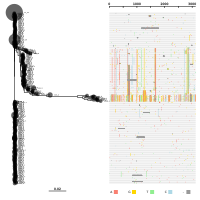
\includegraphics[height=4cm]{images/tree-align.png} 
\end{center}

\end{frame}



\begin{frame}[fragile]
\frametitle{report snakefile }

\alert<1> 

\begin{tiny}
\begin{verbatim}
rule report:
    input:
        "postproc/{dataset}/{sample}/{sample}_qc_bins.png",
        "postproc/{dataset}/{sample}/{sample}_qc_bins.csv",
        "postproc/{dataset}/{sample}/{sample}.fasta.mds.png",
        "postproc/{dataset}/{sample}/{sample}.fasta.tre.svg",
        "postproc/{dataset}/{sample}/{sample}.fasta",
        "postproc/{dataset}/{sample}/{sample}.fasta.rejected.fasta",
        "postproc/{dataset}/{sample}/{sample}.fasta.rejected.csv"
    params:
        VERSION = VERSION,
        COMMIT = COMMIT,
        blast = "true",
        thresh_hold = "0.05",
        max_clades = "5",
        max_waits = "10"
    output:
        "postproc/{dataset}/{sample}/{sample}-report.html",
        "postproc/{dataset}/{sample}/{sample}-blast.csv"
    script:
        "scripts/report.jl"
\end{verbatim}
\end{tiny}

Output from the {\tt postproc} script is fed into the {\tt report}
script and {\tt html} reports are generated and annotated with
explanatory text and version identiiers. blast parameters are
passed in the `params` block

\end{frame}

\subsection{index}

\begin{frame}[fragile]
\frametitle{index }

\alert<1> 

This script generates an `html` index page for the individual sample report pages.

\bigskip
A rejection count summary table for all samples is also presented
to convince the user that all sequences are accounted for.

\end{frame}

\begin{frame}[fragile]
\frametitle{index snakefile }

\alert<1> 

\begin{tiny}
\begin{verbatim}
rule index:
    input:
        expand("postproc/{dataset}/{sample}/{sample}-report.html", zip, dataset = DATASETS, sample = SAMPLES),
        expand("postproc/{dataset}/{sample}/{sample}-blast.csv", zip, dataset = DATASETS, sample = SAMPLES)
    params:
        VERSION = VERSION,
        COMMIT = COMMIT,
        SAMPLES = SAMPLES
    output:
        "postproc/{dataset}/report_index.html",
        "postproc/{dataset}/{dataset}-blast.html"
    script:
        "scripts/index.jl"
\end{verbatim}
\end{tiny}

Output from the {\tt report} script is fed into the {\tt index}
script and an {\tt html} index is generated and annotated with
a summary of rejection counts. 

\end{frame}

\subsection{tar}

\begin{frame}[fragile]
\frametitle{tar}

\alert<1> 

This script archives and compresses the {\tt porpid} and {\tt postproc} output directories
to make it easy for the user to download results from a PORPIDpipeline server.

\begin{tiny}
\begin{verbatim}
rule tar:
    input:
        "postproc/{dataset}/report_index.html"
    output:
         "porpid/{dataset}-porpid.tar.gz",
        "postproc/{dataset}-postproc.tar.gz"
    params:
        degap = "false",
        datasets = DATASETS,
        samples = SAMPLES
    script:
        "scripts/tar.jl"
\end{verbatim}
\end{tiny}

The tar script waits for the index script to complete and then performs the
archiving and zipping process with the help of a Julia script.

\end{frame}

\subsection{blast}

\begin{frame}[fragile]
\frametitle{experimental BLAST pipeline}

\alert<1> 

Finally, a second pipeline is provided for producing BLAST reports
on each sample. If this pipeline is run (after the PORPIDpipeline )
than a BLAST report is generated for representatives of major
clades in each sample.  

\bigskip
If a sample has rejected sequences then the longest sequence in 
the rejected file is appended to the BLAST query.

\bigskip
Note that the BLAST pipeline may have to be re-run many times
in order to generate reports for every sample. This is due to the
transient nature of the public BLAST server and users that rely
on this BLAST facility may want to set up their own dedicated 
server.

\end{frame}

\begin{frame}[fragile]
\frametitle{example BLAST output}

\alert<1> 



\bigskip
\begin{center}
\includegraphics[height=3cm]{images/blast.png} 
\end{center}

\bigskip
a BLAST report that shows the top hit for
each of two clades present in the sample. 

\end{frame}

\section{Installation}

\begin{frame}[fragile]
\frametitle{Installation}

\alert<1> 

The {\tt PorpidPostroc} repository is located at:

\bigskip
{\color{blue} \href{https://github.com/MurrellGroup/PORPIDpipeline}{https://github.com/MurrellGroup/PORPIDpipeline} }

\bigskip
This repository has quick start instructions on how to get PORPIDpipeline up and running
in a minimal environment:

\begin{itemize}
\item installing third party software, {\tt snakemake}, {\tt mafft}, {\tt fasttree}.
\item cloning the PORPIDpipeline repository
\item Installing Julia 1.7
\item setting up the Julia environment for PORPIDpipeline.
\item processing the {\tt demo} data files packaged with PORPIDpipeline.
\end{itemize}

The quick start instructions also point the user to a script that allows full installation
of PORPIDpipeline in a {\em Conda} environment.


\end{frame}

\section{Credits}

\begin{frame}[fragile]
\frametitle{Credits}

\alert<1> 

This introduction to {\em PORPIDpipeline} and the individual script descriptions are based on the 
PORPID-postproc (branch h704)  README written by {\em Alec Pankow}.

\bigskip
\bigskip
The introduction to {\em Snakemake} is based on introductory slides written by {\em Johannes Koester},
the originals of which can be viewed
at \href{http://slides.com/johanneskoester/deck-1}{http://slides.com/johanneskoester/deck-1}.


\end{frame}


\end{document}
